\section*{Dedicated Security Chips}

Computing platform providers have recently added new security chips to their systems. We look at two examples of this pattern: Google's Titan and Apple's T2 chips.

\subsubsection*{Google Titan}

Titan~\cite{titan} is a security chip implemented as a low-power microcontroller on Google's purpose-built server platforms. The Titan chip communicates with the main CPU via the Serial Peripheral Interface (SPI), and it interposes between the boot firmware flash and the Platform Controller Hub (PCH).

 One of the main functionalities that Titan implements is \emph{secure boot}. When the server machine is powered up, Titan executes code, known as boot ROM, from its embedded read-only memory. This code is immutable and thus implicitly trusted. The boot ROM code loads Titan's firmware from the embedded flash and verifies its integrity using a digital signature. Once Titan's firmware is securely verified and running, it can verify the boot process of its host. Titan blocks PCH's access to the firmware flash until it has cryptographically verified the content of the flash, and then it releases the lock and allows the verified boot firmware to configure the machine and load the boot loader which subsequently verifies and loads the OS. Such an iterative process allows precise control over which system software is booted. 

\begin{figure}[t]
    \centering
    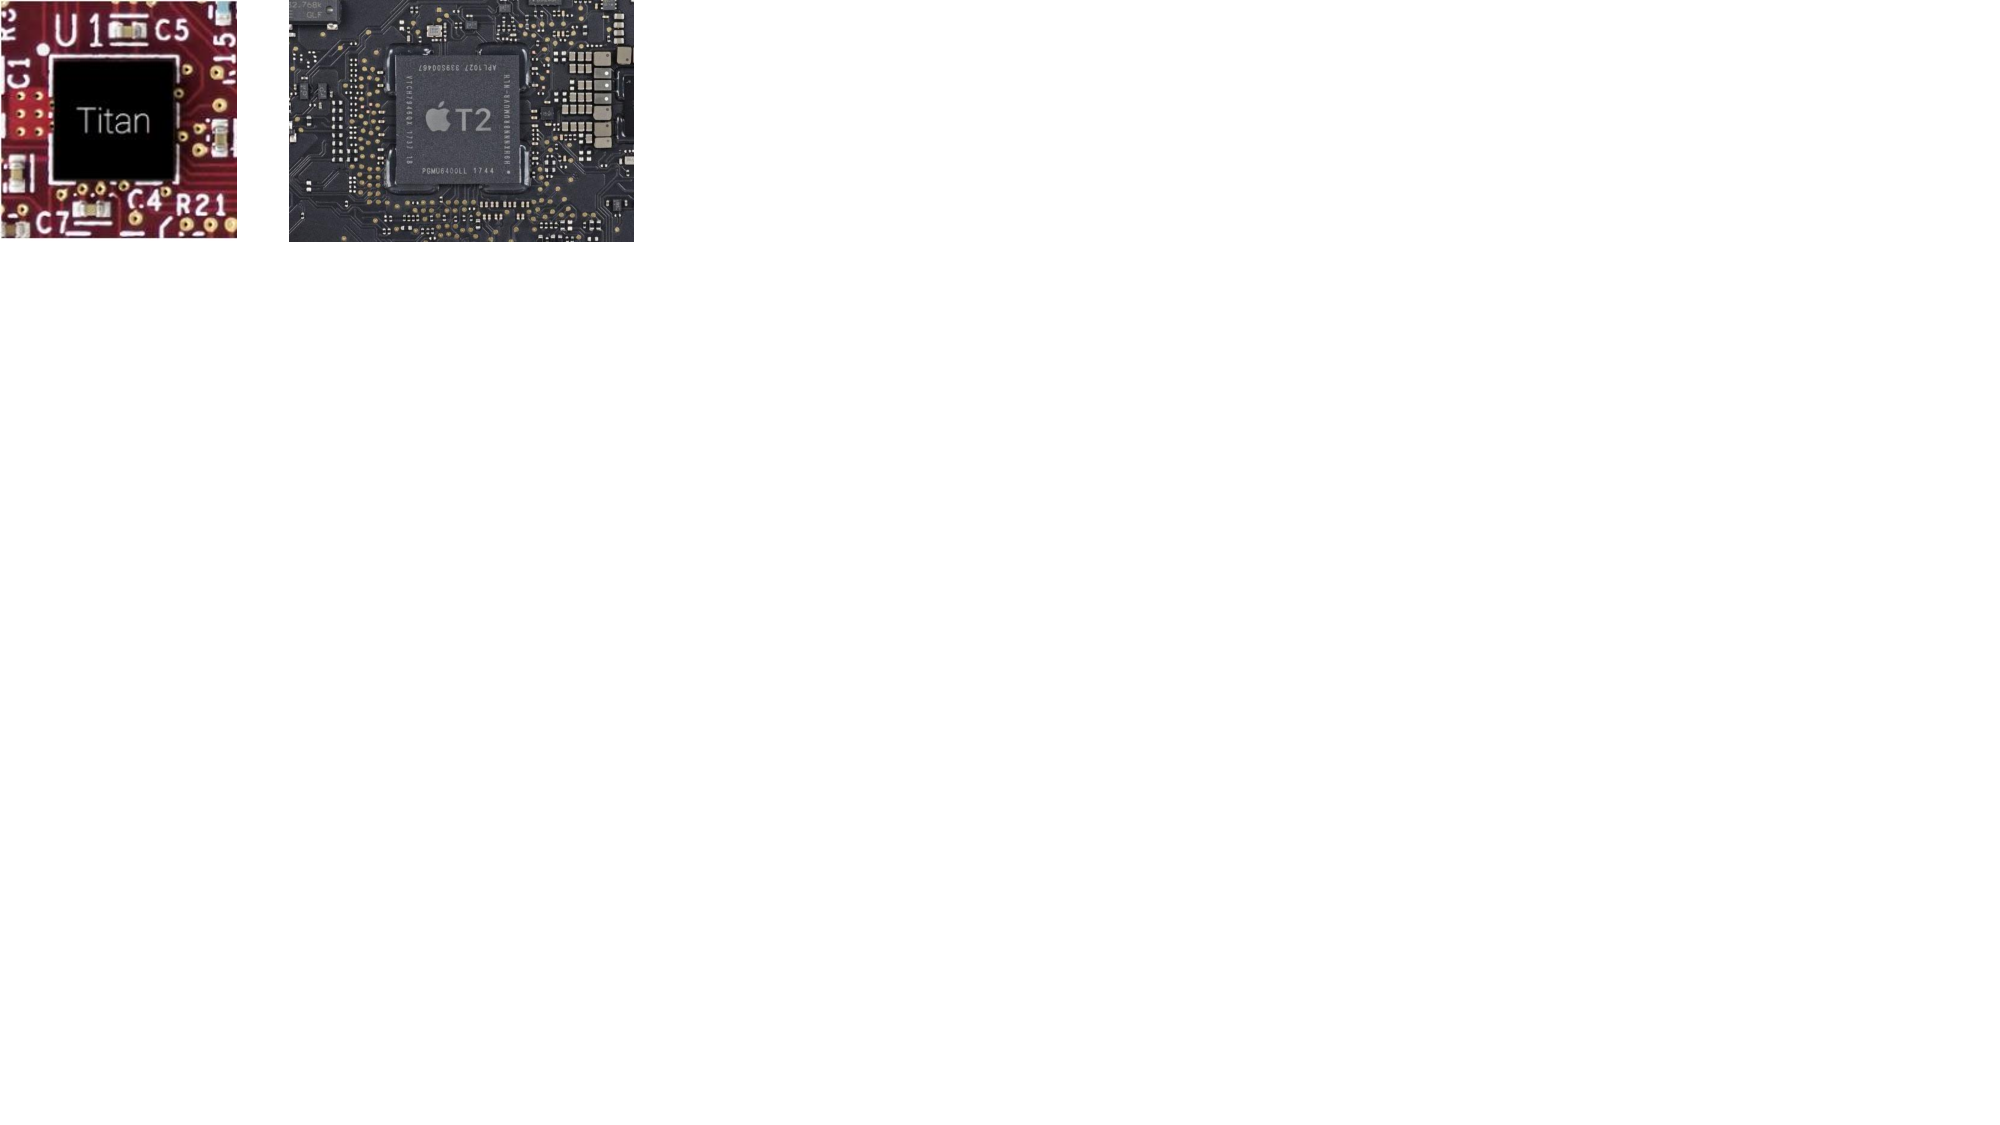
\includegraphics[scale=0.7]{chips.pdf}
    \caption{Google Titan~\cite{titan} and Apple T2~\cite{t2} security chips.}
\label{fig:prototype}   
\end{figure}

 
\subsubsection*{Apple T2}
 
Apple's latest PCs come with a security chip called T2~\cite{t2} that also supports secure boot. When the machine with the T2 chip is turned on, T2 executes code from its read-only memory. This code verifies the next step of the T2's own boot process. Once T2 is fully running, it can verify the UEFI firmware, which will ensure that only authorized kernel will be booted on the host CPU.

Besides secure boot, T2 provides also other security features such as protecting the user's fingerprint values or making sure that the microphone is disconnected from the main CPU when the laptop's lid is closed. 
 
 
\subsubsection*{\update{2}{Specific Security Objectives}}

%In SGX, enclaves are constructed by the untrusted OS. The construction process of the enclave --- that is, the sequence of setup instructions and their parameters --- is recorded by the CPU so that it can be later communicated to an external verifier using the built-in attestation mechanism. This ensures that secrets will be provisioned only to correctly constructed enclave, and the untrusted OS cannot access those secrets. Thus, SGX enclaves are protected from the OS, but they \emph{cannot exist without it}. 
  
Both Titan and T2 implement secure boot. Secure boot is also a good example of a security mechanism \update{2}{that is beyond the security objectives of SGX.}

\update{2}{SGX was designed to provide a specific set of protections. These protections include detection of integrity violation of an enclave instance, confidentiality of enclave's data, isolation between enclaves, and enforcement that enclave's execution always starts from an authorized location~\cite{mckeen2013}.} 

\update{2}{Because the security objectives of SGX do not include OS integrity verification, platform providers have added dedicated security chips, like Titan and T2, to implement such security functionality.} Disconnecting the microphones from the main CPU is another example of a security feature that is not provided by enclaves. (As noted in Textbox 1, other processor-based TEEs like the ARM TrustZone architecture can accommondate secure boot.) 

%% ------------ %%

\begin{figure}
    \begin{tcolorbox}
    \textbf{Textbox 1:} 
    ARM TrustZone is a processor-based TEE architecture that is commonly used on smartphones. The main idea of TrustZone is to implement two separate execution modes on the main CPU. All untrusted software, like the OS and third-party apps, are executed in the \emph{normal world}, while applications that need protection run in a separate execution mode called the \emph{secure world}. The processor and memory controllers ensure that any process in the normal world cannot access the secure world.
    
    \hspace{10pt} TrustZone can enable secure boot~\cite{ekberg2014untapped}. A mobile device can be configured such that when the device is powered up, the main CPU starts executing implicitly trusted code that is loaded from read-only memory in secure world. This code can then verify the normal world boot loader before the CPU starts executing the main boot sequence of the normal world OS. Many smartphone manufacturers implement this approach.
	\end{tcolorbox}
\end{figure}  

%% ------------ %%

\subsubsection*{Security Weaknesses}

Besides missing functionality, enclaves also have security weaknesses. Since enclaves and untrusted code share the same CPU, they can be susceptible to side-channel leakage and microarchitectural attacks. The recently discovered Spectre and Meltdown vulnerabilities showed how transient execution could leak information across isolation boundaries. The same idea was successfully applied to extract secret keys from SGX enclaves in the Foreshadow attack~\cite{van2018foreshadow}. 

While specific attacks can be, and have been, mitigated (e.g., Intel's microcode updates include Spectre and Meltdown patches), side-channels and microarchitectural attacks continue to be a concern for enclaves. The root cause is that modern processors are extremely complex systems that have been optimized over decades. Enclave support was added on top of many layers of performance optimizations, and now, in hindsight, one can easily say that this approach was not the ideal foundation for strong isolation. In this regard, dedicated security chips have a clear advantage over enclaves.

Another security challenge is the rich interface between the untrusted OS and the enclave. Enclaves must interact with the operating system in many ways. For example, enclaves communicate by sending and receiving messages through the OS. Enclaves also need to safely pause their execution for interrupts. While enclave architectures provide coarse-grained memory isolation primitive at the hardware level, developers need to ensure that the interface is protected on the software level. Common implementation tasks include sanitization of buffers and safety checks for pointers. 

Because such checks are tedious, several enclave runtimes like the Open Enclave SDK have been developed to assist enclave developers. However, recent research has shown that many such enclave runtimes have classical memory safety vulnerabilities~\cite{van2019tale}. Because dedicated security chips do not need equally extensive interaction with the OS, the interface towards the untrusted OS is easier to protect tightly. 


\subsubsection*{Other Security Services?}

To summarize our discussion so far, enclaves cannot implement all useful platform security mechanisms, and they have significant security issues. Dedicated security chips can address both of these concerns. 

Obviously, the security services that can be implemented as dedicated security chips are not limited to the above-discussed examples. Which other services could be implemented as special-purpose security chips? 

Titan and T2 are integrated security chips that are permanently attached to the computing platform. Are there also use cases that would benefit from plug-and-play security tokens?

In the rest of this article, we explore these questions by examining two case studies from our recent research. Our first case is trusted path~\cite{protection}, \red{\#R1 where we explore how dedicated security chips enable trusted path to untrusted platform} and after that we focus on TEE identification and remote attestation~\cite{proximitee} \red{that uses a dedicated external hardware in order to harden the Intel SGX's remote attestation}.
